\documentclass{ctexart}
\usepackage[left=1.5cm,right=1.5cm,top=1.5cm,bottom=1.5cm]{geometry}
\usepackage{listings}
\usepackage[dvipsnames]{xcolor}
\usepackage{cite}
\usepackage{diagbox}
\usepackage{fancyhdr} % 加载fancyhdr宏包,用于设置页眉和页脚
\pagestyle{fancy} % 设置页面样式
\fancyhf{} % 清除默认的页眉和页脚的内容
\fancyfoot[C]{\thepage} 
\renewcommand{\headrulewidth}{0pt} % 将页眉的横线宽度设置为0pt

\usepackage{graphicx}
\usepackage{longtable}
\usepackage{tabularx}
\usepackage{float}
\usepackage{amsmath}%引用宏包要放在documentclass后面,否则报错
\usepackage{hyperref}
\usepackage{bm}
\usepackage{amssymb}
\usepackage{esint}
\usepackage{booktabs}
%\usepackage{subfiles}%用于分章节管理引用,使各章节引用来源于各自的文件,编号相互独立
\usepackage{amsthm}
\title{数字电路实验\quad 实验报告6}
\author{Leo}
\date{\today}
\begin{document}
\maketitle
\section{实验内容}
使用74194和74138设计序列信号发生器,产生两组不同序列:\\
1.熟悉74194和74138芯片\\
2.列出状态转移真值表和转换图\\ 
3.给出电路实现方案\\
4.调试电路,根据自己的学号最后两位,实现两组不同的周期序列:当控制信号X=0时,输出学号后两位对应的6位二进制数,当X=1时,输出学号后两位对应的在模为50的6位二进制补数。
\section{实验器材}
Pocketlab、电脑、导线若干、镊子、限流电阻1个、红色LED灯1个、7400*1、7404*1、7420*1、74138*1、74194*1。部分芯片的引脚图如下所示
\begin{figure}[H]
    \centering
    \begin{minipage}{0.5\textwidth}
    \centering
           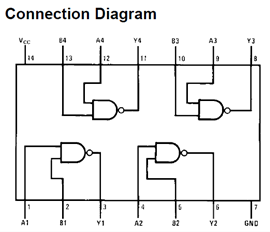
\includegraphics[width=0.6\textwidth]{7400.png}
           \caption{7400}
    \label{}
    \end{minipage}
    \hspace{0.05\textwidth}
    \begin{minipage}{0.3\textwidth}
    \centering
           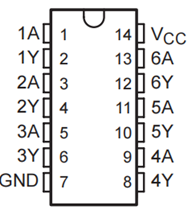
\includegraphics[width=0.6\textwidth]{7404.png}
           \caption{7404}
    \label{7474}
    \end{minipage}
\end{figure}

\begin{figure}[H]
    \centering
    \begin{minipage}{0.5\textwidth}
    \centering
           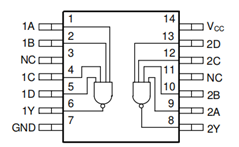
\includegraphics[width=0.6\textwidth]{7420.png}
           \caption{7420}
    \label{}
    \end{minipage}
    \hspace{0.05\textwidth}
    \begin{minipage}{0.3\textwidth}
    \centering
           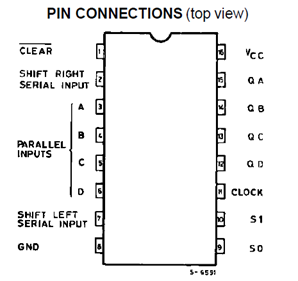
\includegraphics[width=0.8\textwidth]{74194.png}
           \caption{74194}
    \label{}
    \end{minipage}
\end{figure}
\section{实验原理}
实验要求通过X的取值实现两种不同的序列输出。两个序列的长度均为6,因此需要一个模为6的计数器,可以考虑使用移位寄存器实现。若用扭环式循环计数器,则对n位寄存器,可以实现一个周期包含2n个状态。因为74194一共有4位,所以取其中三位即可实现既定功能。按照扭环计数器的设计思路,写出如下状态转移真值表
\begin{table}[H]
    \centering
    \caption{状态转移真值表}
    \begin{tabular}{cccccc}
    \hline 
        $Q_0^n$ & $Q_1^n$ & $Q_2^n$ & $Q_0^{n+1}$ & $Q_1^{n+1}$ & $Q_2^{n+1}$ \\ \hline 
        0 & 0 & 0 & 1 & 0 & 0 \\
        1 & 0 & 0 & 1 & 1 & 0\\
        1 & 1 & 0 & 1 & 1 & 1 \\
        1 & 1 & 1 & 0 & 1 & 1\\ 
        0 & 1 & 1 & 0 & 0 & 1\\ 
        0 & 0 & 1 & 0 & 0 & 0\\ \hline
    \end{tabular}
    \label{状态转移真值表}
\end{table}
可以写出对应的状态转移方程
\begin{equation}\label{1}
    D_{SR}=Q_2'^{n}
\end{equation}
此时控制端$S_0S_1=10$,这样才能实现右移。接下来检查电路自启动,可以将所有8种状态列成状态转换图
\begin{figure}[H]
    \centering
    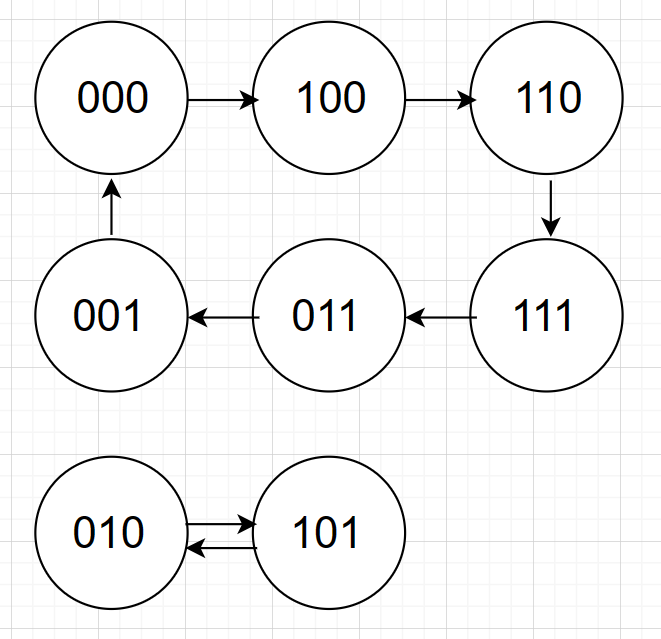
\includegraphics[width=0.4\textwidth]{不能自启动.png}
\end{figure}
发现该电路不能自启动,需要修正。考察010和101两种状态,若将101的次态调整为主循环中的一种情况,则电路可以自启动。不妨将式\ref{1}修改为
\begin{equation}
    D_{SR}=Q_2'^{n}+Q_0^n Q_1'^{n} Q_2^n
\end{equation}
修正后的状态转换图为
\begin{figure}[H]
    \centering
    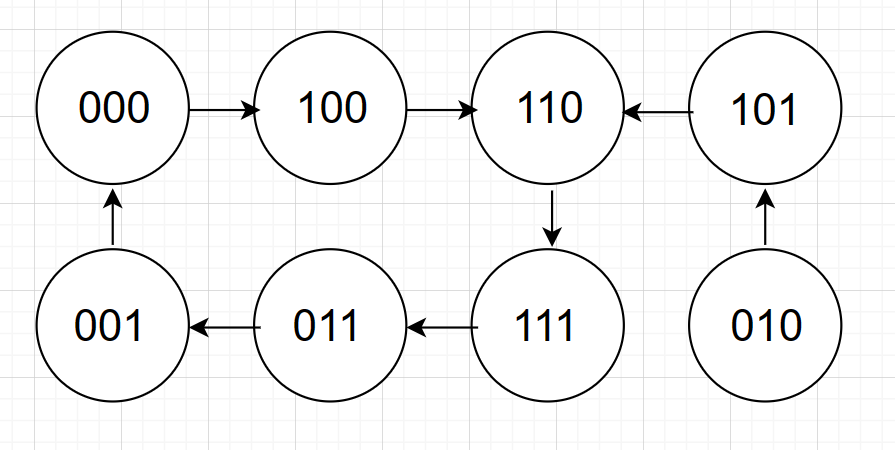
\includegraphics[width=0.5\textwidth]{自启动.png}
\end{figure}
借助74138和7420,可以很方便地完成这个修正。下面列出完整的状态转移真值表,包括输入和对应的输出。
\begin{table}[H]
    \centering
    \caption{状态转移真值表}
    \begin{tabular}{cccccccc}
    \hline 
        $Q_0^n$ & $Q_1^n$ & $Q_2^n$ & $Q_0^{n+1}$ & $Q_1^{n+1}$ & $Q_2^{n+1}$ & X & Z\\ \hline 
        0 & 0 & 0 & 1 & 0 & 0 & 0 & 0\\
        1 & 0 & 0 & 1 & 1 & 0 & 0 & 0\\
        1 & 1 & 0 & 1 & 1 & 1 & 0 & 1\\
        1 & 1 & 1 & 0 & 1 & 1 & 0 & 1\\ 
        0 & 1 & 1 & 0 & 0 & 1 & 0 & 0\\ 
        0 & 0 & 1 & 0 & 0 & 0 & 0 & 1\\ 
        0 & 1 & 0 & 1 & 0 & 1 & 0 & x\\
        1 & 0 & 1 & 1 & 1 & 0 & 0 & x\\
        0 & 0 & 0 & 1 & 0 & 0 & 1 & 1\\
        1 & 0 & 0 & 1 & 1 & 0 & 1 & 0\\
        1 & 1 & 0 & 1 & 1 & 1 & 1 & 0\\
        1 & 1 & 1 & 0 & 1 & 1 & 1 & 1\\ 
        0 & 1 & 1 & 0 & 0 & 1 & 1 & 0\\ 
        0 & 0 & 1 & 0 & 0 & 0 & 1 & 1\\ 
        0 & 1 & 0 & 1 & 0 & 1 & 0 & x\\
        1 & 0 & 1 & 1 & 1 & 0 & 0 & x\\ \hline
    \end{tabular}
    \label{完整的状态转移真值表}
\end{table}
图中两种偏离状态的输出可以视作无关项。借助状态转移真值表可以做出卡诺图
\begin{table}[H]
    \centering
    \caption{X=0时的卡诺图}
    \begin{tabular}{|c|c|c|c|c|}
\hline
\diagbox{$Q_0$}{$Q_1Q_2$} & 00 & 01 & 11 & 10 \\
\hline
0 & 1 & 0 & 1 & x \\
\hline
1 & 0 & x & 1 & 0  \\
\hline
\end{tabular}
    \label{X=0时的卡诺图卡诺图}
\end{table}
\begin{table}[H]
    \centering
    \caption{X=1时的卡诺图}
    \begin{tabular}{|c|c|c|c|c|}
\hline
\diagbox{$Q_0$}{$Q_1Q_2$} & 00 & 01 & 11 & 10 \\
\hline
0 & 1 & 0 & 1 & x \\
\hline
1 & 1 & x & 0 & 0  \\
\hline
\end{tabular}
    \label{X=1时的卡诺图}
\end{table}
根据卡诺图可以写出输出$Z$关于$Q_0Q_1Q_2X$的表达式
\begin{align}
    Z&=X'(Q_0'Q_2'+Q_1Q_2)+X(Q_1'Q_2'+Q_0'Q_1)\\
    &=X'\sum m(0,2,3,7)+X\sum m(0,2,3,4)
\end{align}
接下来可以进行电路仿真和测试了。
\section{电路实现与调试}
在Multisim中搭建上文所述的电路
\begin{figure}[H]
    \centering
    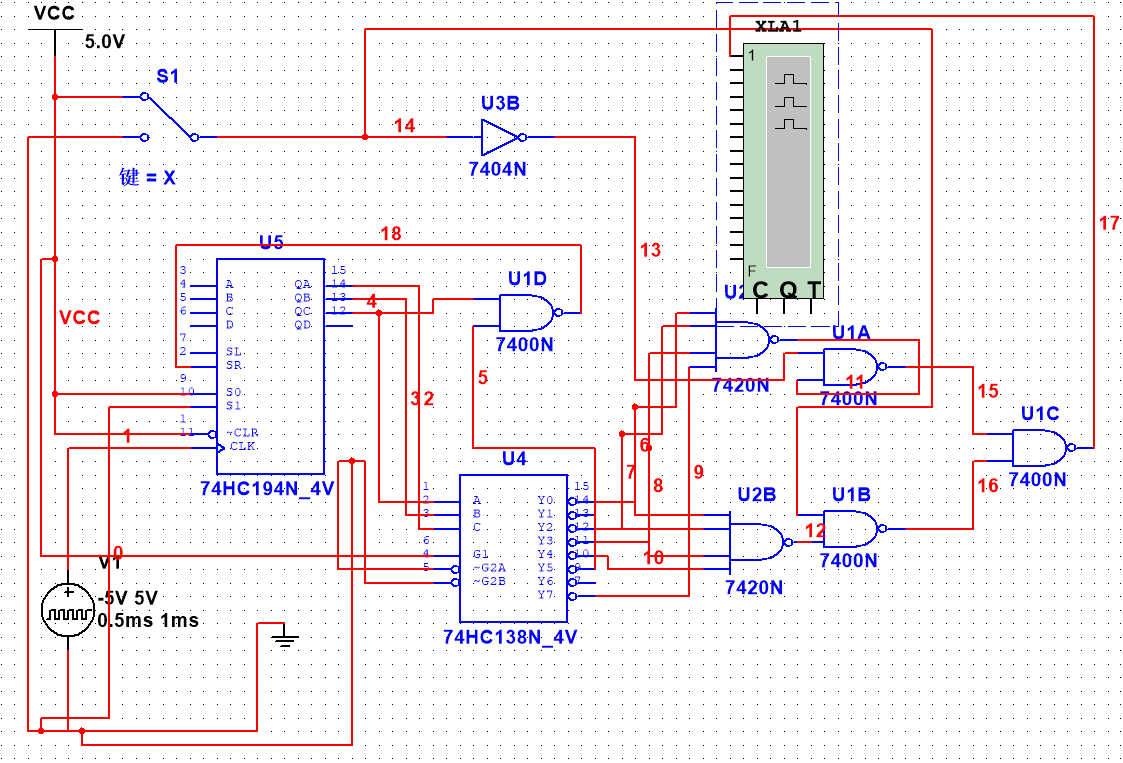
\includegraphics[width=0.6\textwidth]{仿真电路图.png}
\end{figure}
采用字发生器检测输出,当X输入为1时,字发生器显示为
\begin{figure}[H]
    \centering
    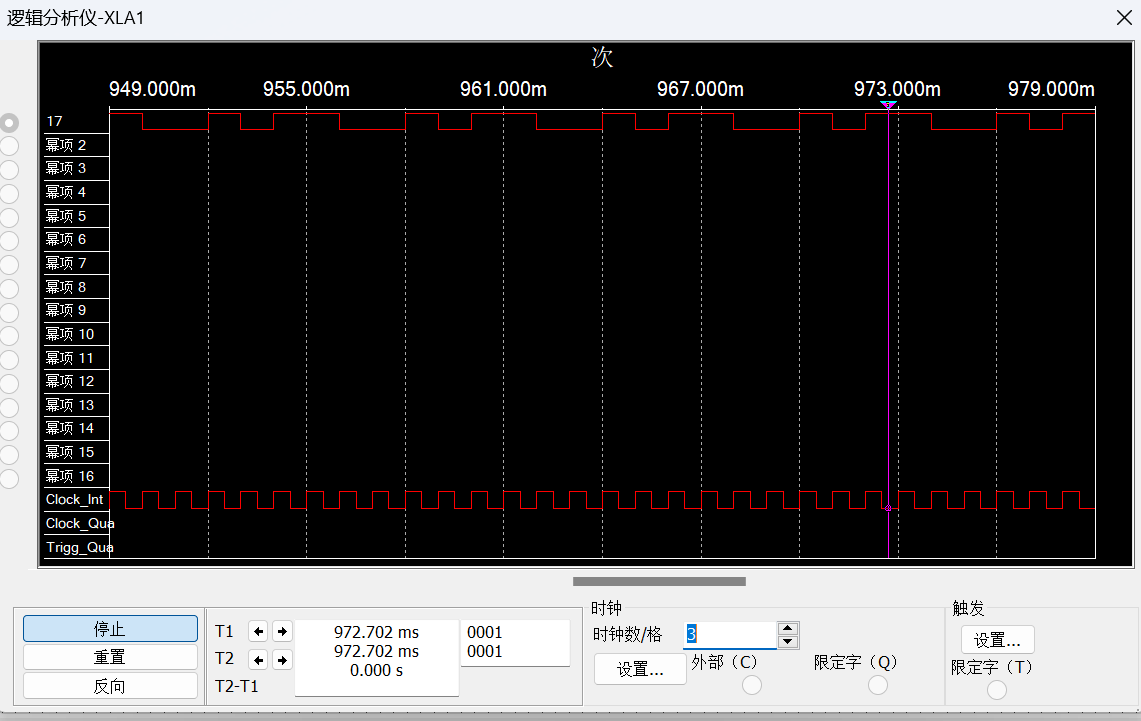
\includegraphics[width=0.6\textwidth]{x=1.png}
\end{figure}
即100101序列。\\
当X输入为0时,字发生器显示为
\begin{figure}[H]
    \centering
    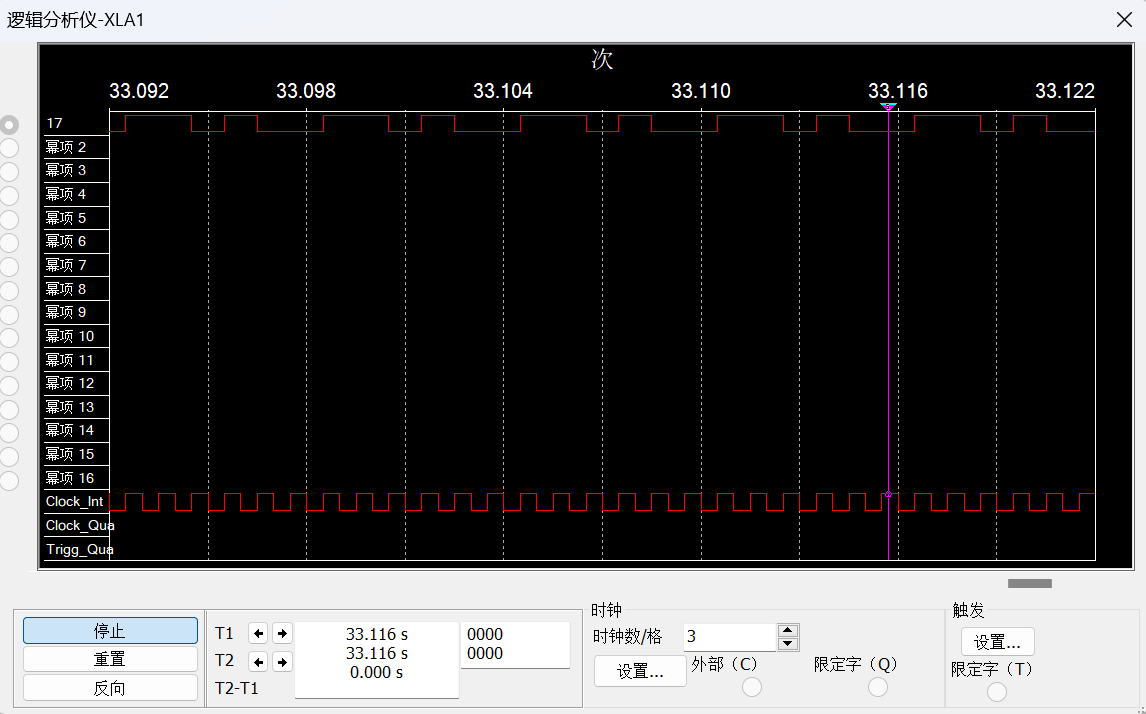
\includegraphics[width=0.6\textwidth]{x=0.png}
\end{figure}
即001101序列。上面的结果说明仿真成功,达到既定效果。\\
下面搭建实物电路图。
\begin{figure}[H]
    \centering
    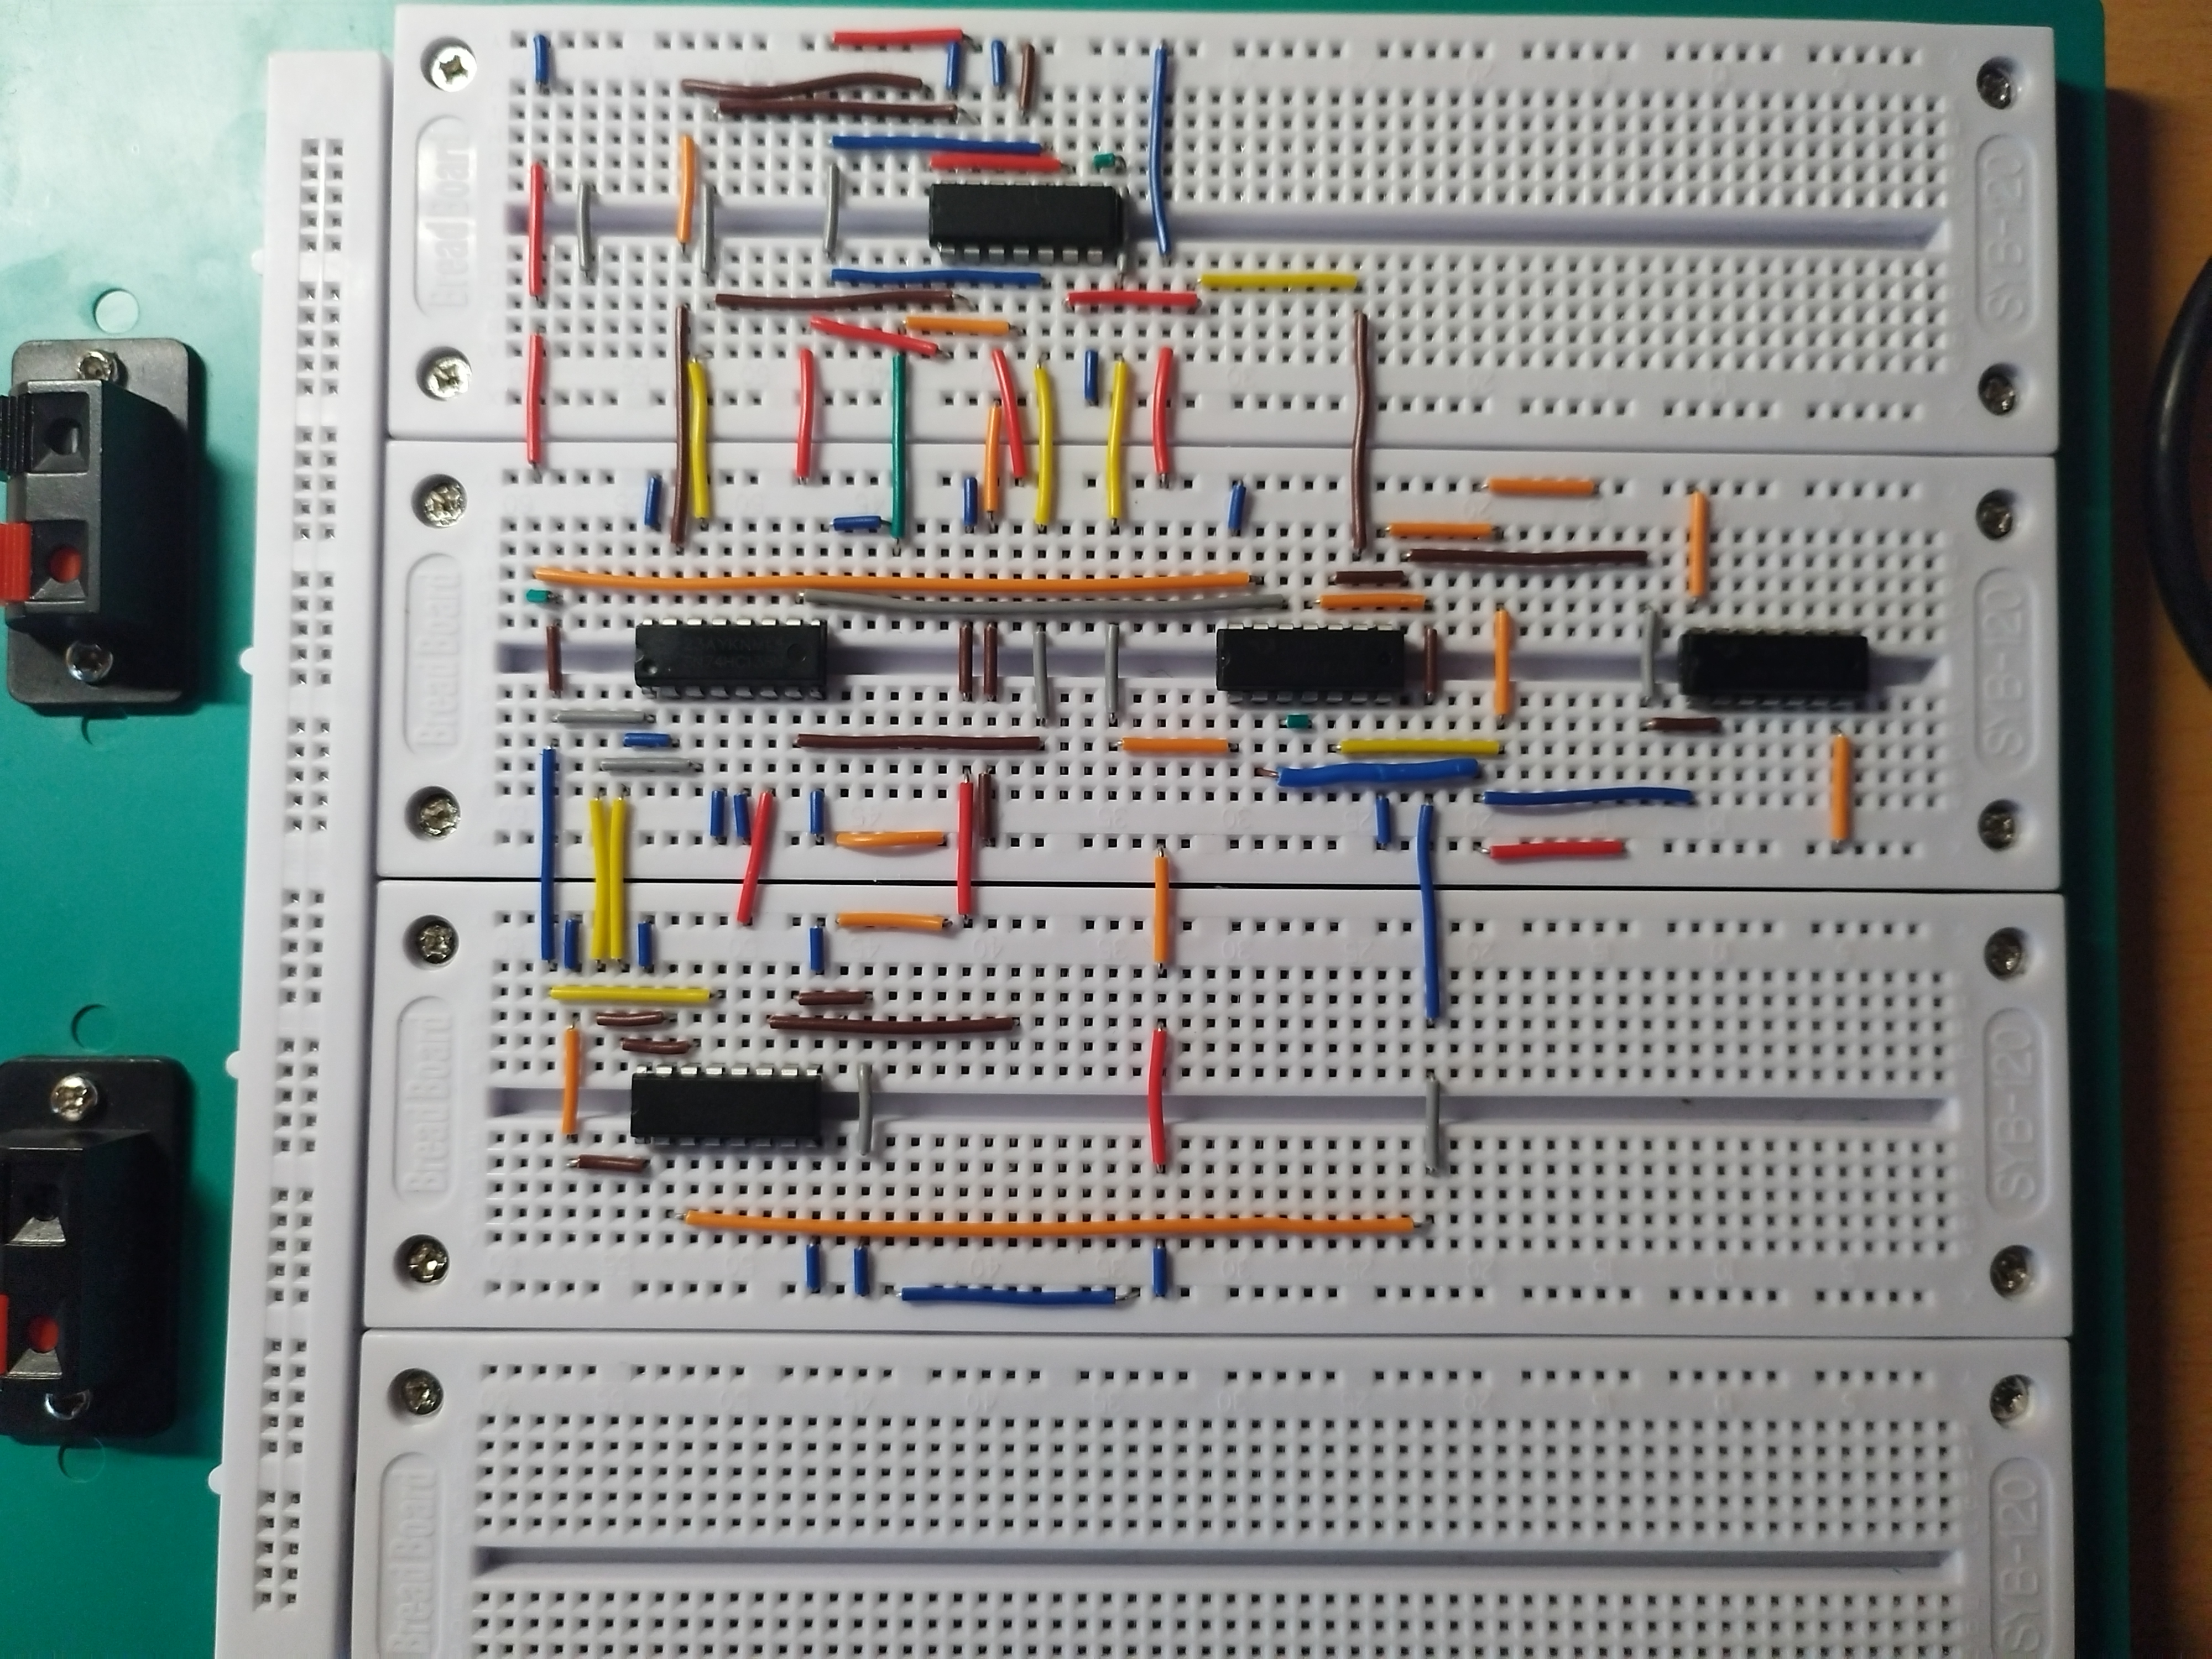
\includegraphics[width=0.6\textwidth]{实物图.jpg}
\end{figure}
通过pocketlab逻辑分析仪查看电路工作是否正常,下面分别是控制信号$x=0,x=1$时的界面截图(一张图不能完整显示一个周期,所以分成两次截图)
\begin{figure}[H]
    \centering
    \begin{minipage}{0.4\textwidth}
        \begin{figure}[H]
            \centering
            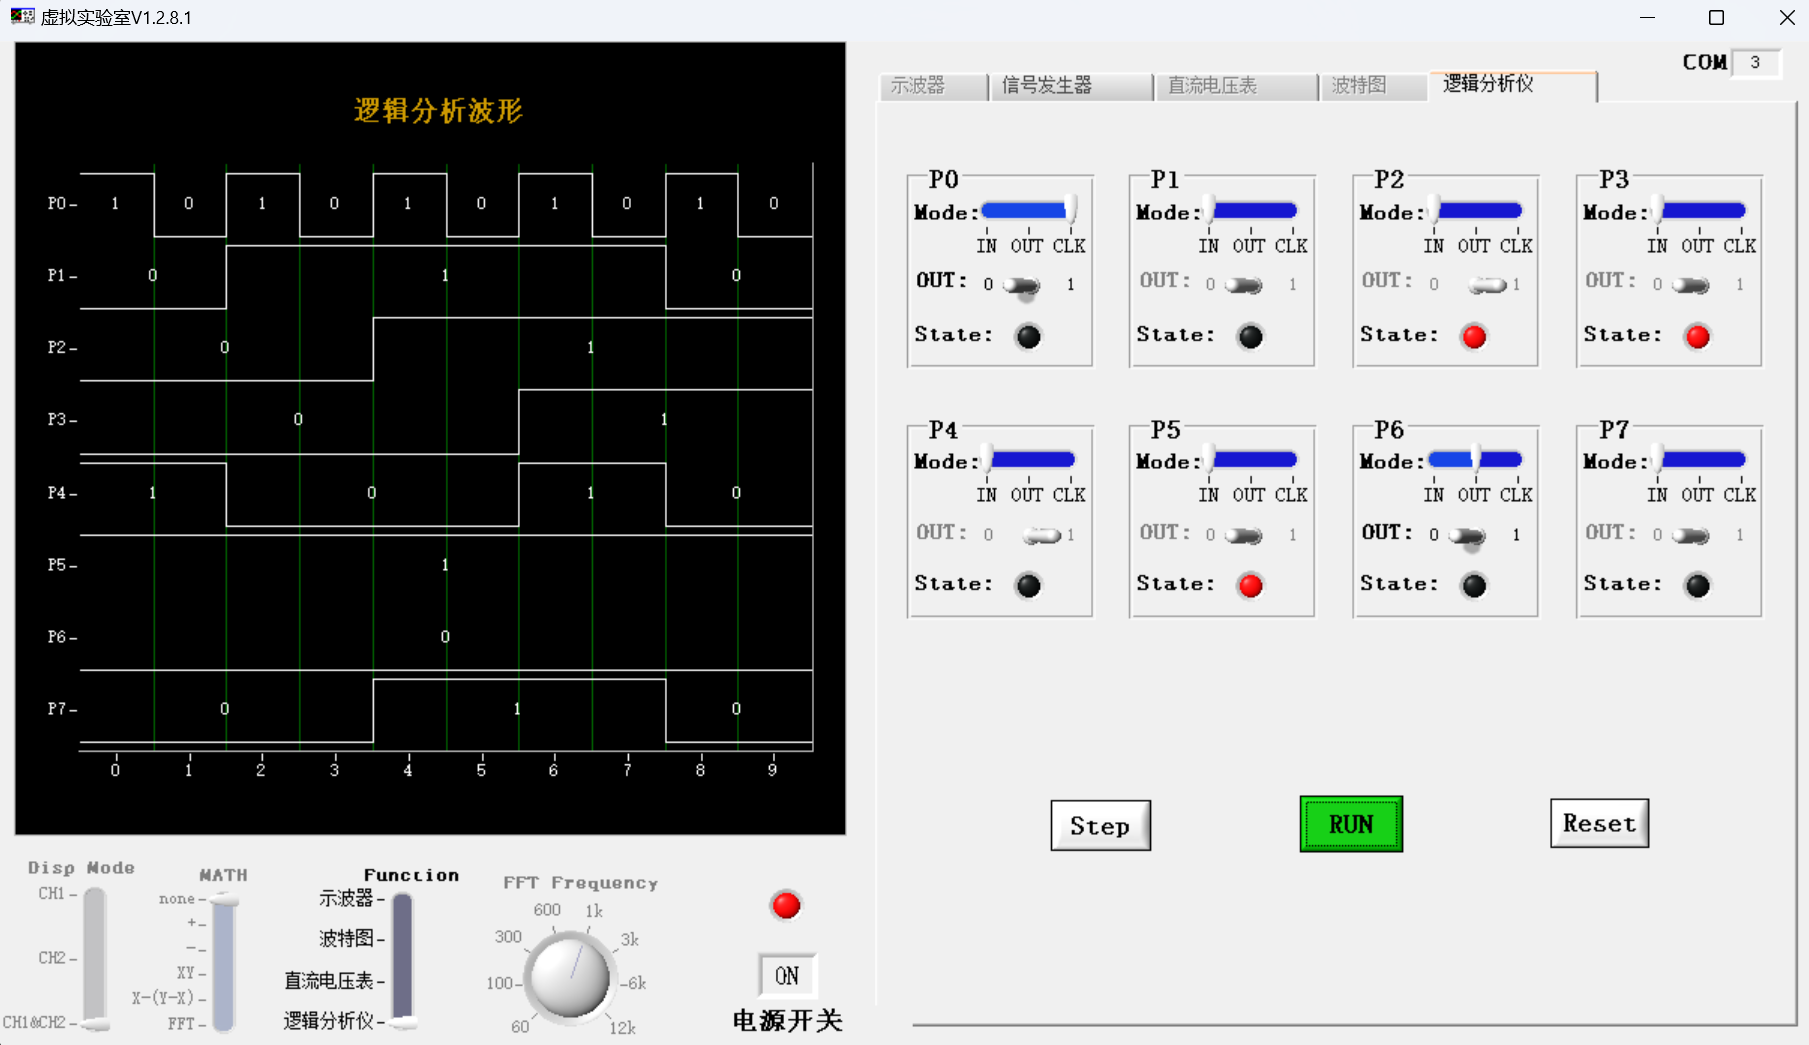
\includegraphics[width=\textwidth]{x=0_1.png}
            \caption{$x=0$截图1}
        \end{figure}
    \end{minipage}
    \hspace{0.1\textwidth}
    \begin{minipage}{0.4\textwidth}
        \begin{figure}[H]
            \centering
            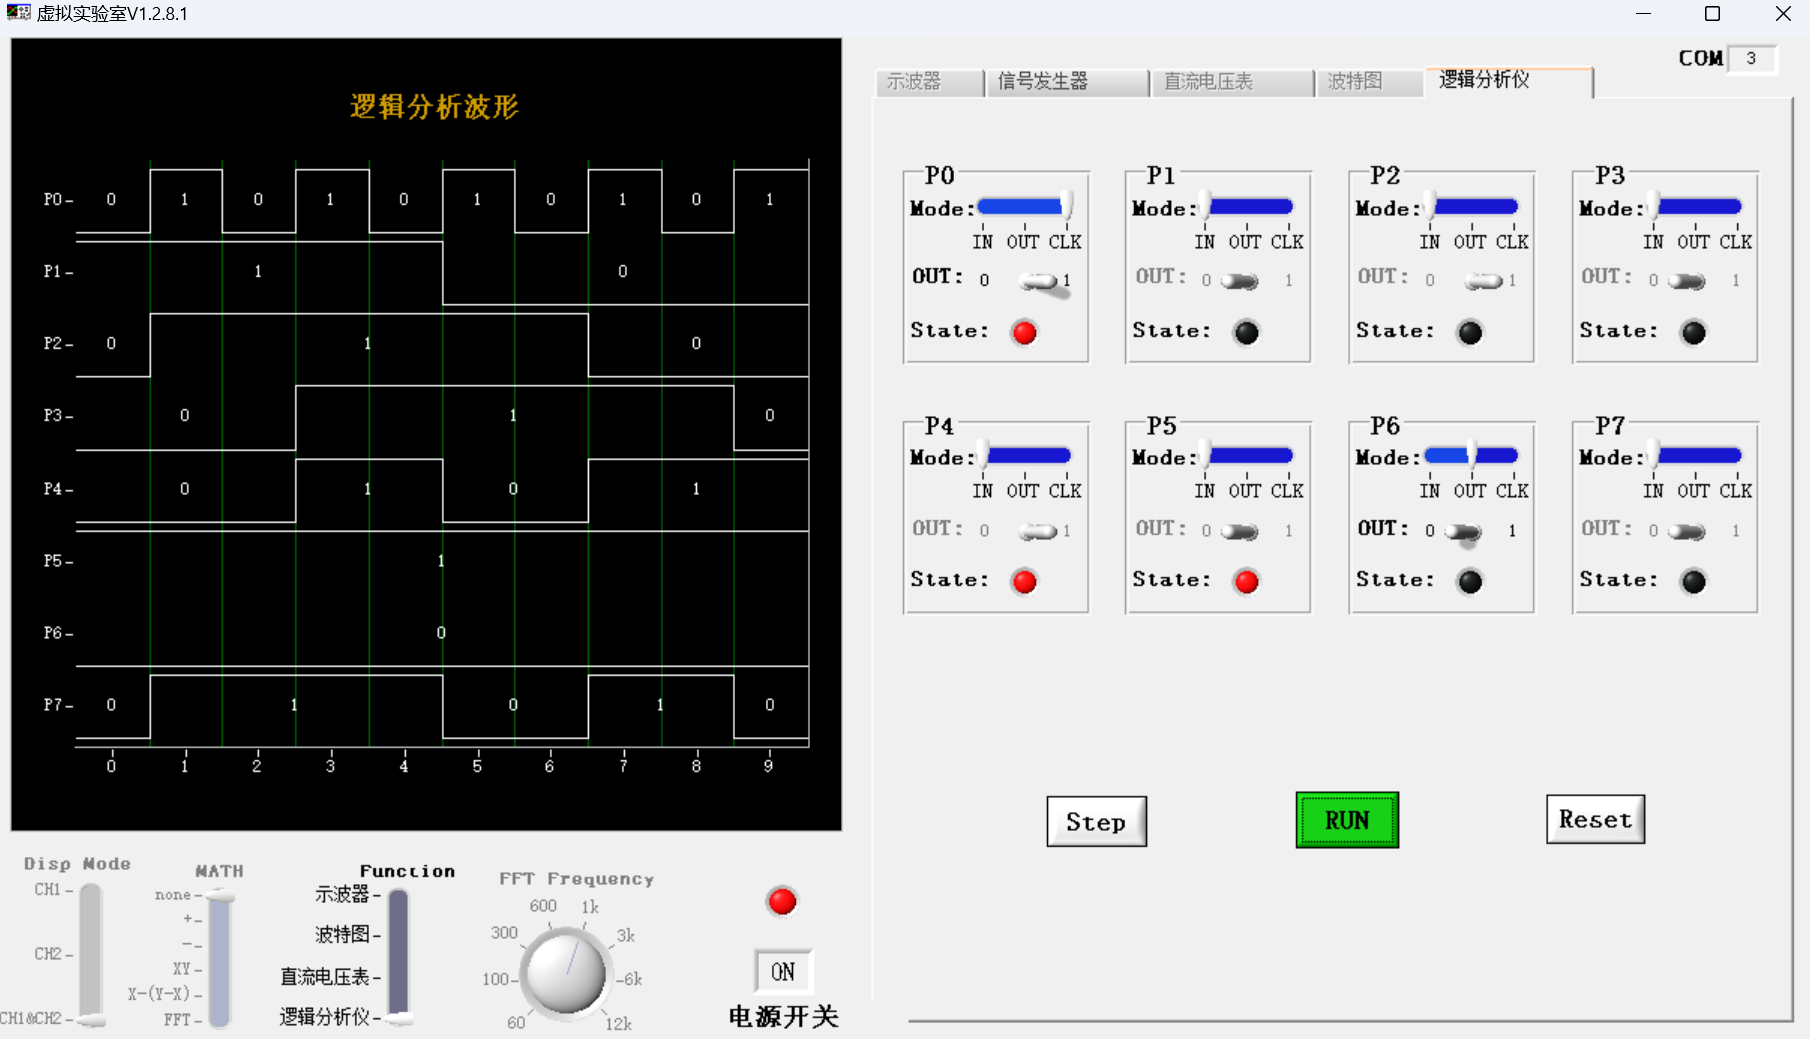
\includegraphics[width=\textwidth]{x=0_2.png}
            \caption{$x=0$截图2}
        \end{figure}
    \end{minipage}
\end{figure}
\begin{figure}[H]
    \centering
    \begin{minipage}{0.4\textwidth}
        \begin{figure}[H]
            \centering
            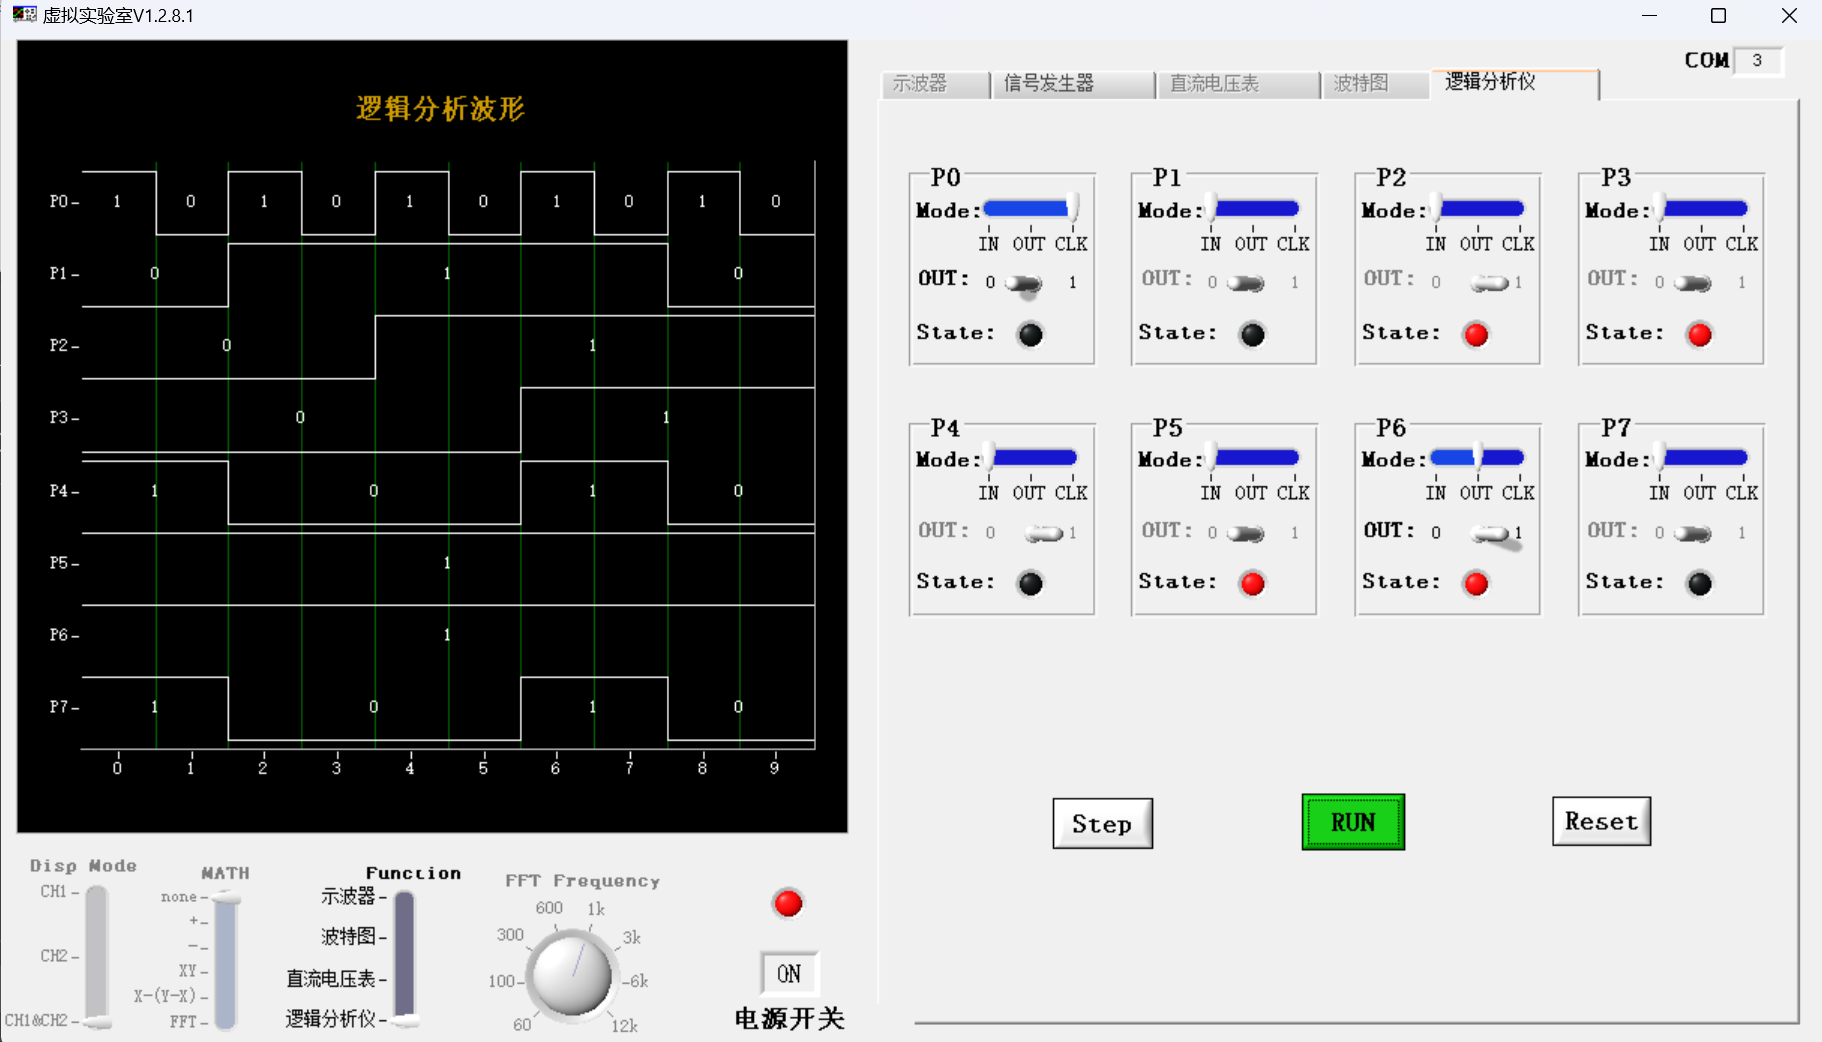
\includegraphics[width=\textwidth]{x=1_1.png}
            \caption{$x=1$截图1}
        \end{figure}
    \end{minipage}
    \hspace{0.1\textwidth}
    \begin{minipage}{0.4\textwidth}
        \begin{figure}[H]
            \centering
            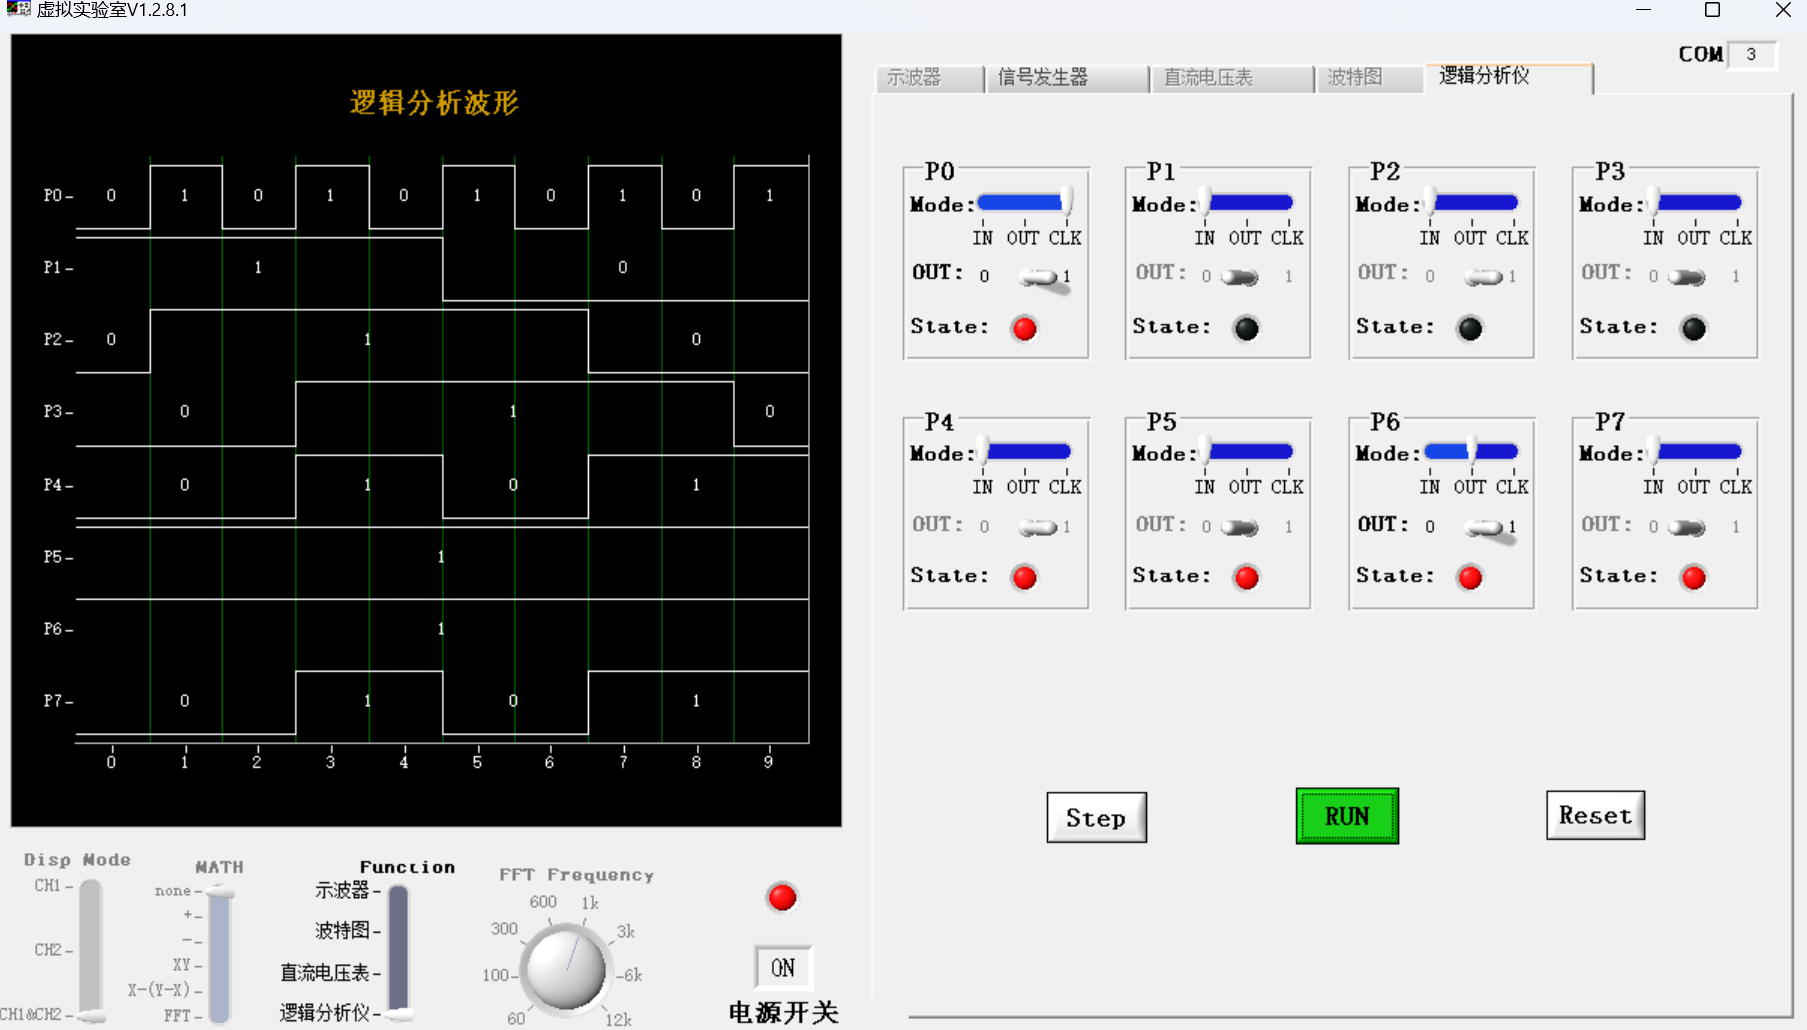
\includegraphics[width=\textwidth]{x=1_2.png}
            \caption{$x=1$截图2}
        \end{figure}
    \end{minipage}
\end{figure}
\section{反思与总结}
本次实验较为顺利,只是在第一遍设计电路时没有检查电路自启动,在画状态转换图时才想起来。这说明在电路设计中每一步流程都是有必要的,可以提醒设计者检查一些不易被发现的电路缺陷。并且,在修正状态转移方程时并没有将式子化到最简,而是借助已有的74138闲置引脚和闲置的7400与非门来实现,而没有引入新的芯片,体现了电路设计的最小化要求。
\end{document}